\chapter{可解释性入门}\label{可解释性入门}

大模型能够生成复杂回答，研究者也希望理解这些行为对应的内部计算。可解释性研究由此连接两个问题：模型的表示中包含什么信息，这些信息怎样参与预测。在学术研究中，相关方法从输入特征归因、表示探针和注意力分析，逐步扩展到激活干预、计算回路发现与稀疏特征分解。研究对象也从小模型上的可控任务，扩展到大语言模型中的知识提取、关系判断与多步生成。

工业界对这条路线同时存在投入与质疑。Anthropic 等企业研究团队持续研究特征提取与计算路径追踪，希望把内部分析用于模型诊断、行为监测和定向调整。面向产品落地的质疑则集中在实际收益：分析一个行为需要多少计算与人工，发现的特征能否在新输入和模型版本上复现，内部干预相对于直接评测、数据改进和重新训练带来多少增益。Google Research 的相关工作也将应用目标和评估指标的标准化，列为判断可解释性方法实用价值的重要问题。

可解释性的潜力在于把输出差异追踪到具体表示与计算路径，为错误定位、训练诊断和模型控制提供更细的实验依据。当前的主要局限是分析覆盖范围、解释粒度与研究成本：局部回路通常围绕特定任务建立，稀疏特征的描述需要样本与干预验证，大模型的激活采集和分析也需要额外资源。因而，本章从可重复的小实验入手，依次介绍信息读出、状态替换和特征分解，让读者掌握提出机制假设并检验它的基本方法。

\textbf{引入阅读}
\begin{enumerate}
    \item Anthropic，2025，\href{https://www.anthropic.com/research/tracing-thoughts-language-model}{Tracing the thoughts of a large language model}。阅读重点：计算路径追踪的研究进展、应用动机与分析成本。
    \item \href{https://research.google/pubs/towards-unifying-interpretability-and-control-evaluation-via-intervention/}{Towards unifying interpretability and control: Evaluation via intervention}。阅读重点：以可测量的干预效果评估可解释性方法的实用价值。
\end{enumerate}

\section{可解释性的证据~看到了什么与证明了什么}\label{可解释性的证据 看到了什么与证明了什么}

前面的训练诊断让我们发现：小助的回答变短，可能只是行为倾向变化；一个词生成不出来，也可能涉及输出端偏移。我们已经能通过输入与输出比较排除一些解释，但还会追问：模型内部到底利用了哪些信息，又通过什么计算形成这次答案？这就是可解释性（interpretability）要帮助我们研究的问题。

我们先区分两个尺度。行为分析改变提示、数据或工具，观察系统如何反应；机制可解释性（mechanistic interpretability）进一步研究参数、激活与计算路径，尝试用可检验的机制解释特定行为。解释的对象可以是一道题、一个注意力头，也可以是跨一批输入反复出现的计算模式。实验开始时写明模型、输入类型与目标行为，后续观察和干预围绕这些对象展开。

最容易上手的是注意力热图。假设小助生成``她''时，一个头对某个人名分配较大权重，这是一条有价值的观察。权重描述该注意力头混合各位置值向量的比例。分析这个头对答案的作用，还需要结合值向量的内容、输出投影、残差流和后续层的计算。热图提供候选位置，针对这些位置的干预实验进一步检验它们对输出的影响。

小助还可以自己解释：``我先根据代词找到人名，再回答。''这段文字描述了模型给出的解题过程，可以帮助读者检查步骤、提出机制假设。研究者再通过改变人名、代词和中间激活，比较回答变化，检验文字解释与实际计算之间的对应关系。

我们把证据分成三层：观察到某个激活与行为相关；从表示中读出某类信息；干预某处计算后，目标行为按预测改变。相关性分析用于发现候选，读出实验用于检查表示中的信息，干预实验用于检验计算对行为的影响。接下来依次介绍读出与受控干预。

\textbf{本节相关资料}
\begin{enumerate}
    \item Jain 与 Wallace，2019，\href{https://arxiv.org/abs/1902.10186}{Attention is not Explanation} 。阅读重点：注意力权重、预测结果与干预效果之间的关系。
    \item Turpin 等，2023，\href{https://arxiv.org/abs/2305.04388}{Language Models Don't Always Say What They Think Unfaithful Explanations in Chain-of-Thought Prompting} 。阅读重点：解释文本如何遗漏实际影响回答的因素。
\end{enumerate}

\section{线性探针 表示中能读出什么}\label{线性探针 表示中能读出什么}

我们怀疑小助在某一层已经表示了``谁把物品给了谁''，但最后没有选对人名。怎样判断信息是在中途丢失，还是存在却没有被后续计算有效利用？一种入门办法是在线性探针（linear probe）上做实验：冻结模型，只训练一个很小的读出器。

\textbf{先定义标签：谁是物品接收者}~标签由研究者根据任务定义并标注。这里把句子中第一次出现的两个人名依次记为人物 1、人物 2，并规定：接收者是人物 1 时，标签 $c=0$；接收者是人物 2 时，标签 $c=1$。例如：
\begin{itemize}
    \item ``小明把书交给了小红。''人物 1 是小明，人物 2 是小红，接收者是小红，因此标签为 1。
    \item ``小明从小红那里收到了书。''人物顺序相同，接收者是小明，因此标签为 0。
    \item ``小红把笔递给了小明。''人物 1 是小红，人物 2 是小明，接收者是小明，因此标签为 1。
    \item ``小红从小明那里接过了笔。''人物顺序相同，接收者是小红，因此标签为 0。
\end{itemize}
这个标签把句子的人物关系变成了一个二分类任务。人物编号按每个句子的出现顺序确定，类别 0 和类别 1 分别对应第一位和第二位人物。更换姓名和物品后，标注规则保持一致。

\textbf{输入探针的是什么}~把完整句子送入冻结的语言模型，取第 $l$ 层、句末最后一个有效 token 位置的隐藏向量 $h$。这里 $l$ 是选定的层编号，$h$ 是一个 $d$ 维向量，$d$ 是模型隐藏维度。因果语言模型在句末位置已经能够读取此前整句，因此这个位置适合用来检查接收者信息。每个句子产生一对训练数据 $(h,c)$：$h$ 来自语言模型，$c$ 来自事先确定的关系标注。只把句子送入语言模型，标签用于探针的损失计算。

\textbf{探针本身需要训练}~线性探针是在隐藏向量上训练的分类器。为每个句子提取 $h$ 后，随机初始化分类器的权重 $W$ 和偏置 $b$，再用带标签的数据学习如何读取这些向量。类别概率写为：
\[
P_\phi(c\mid h)=\operatorname{softmax}(Wh+b)_c.
\]
这里，$W\in\mathbb R^{2\times d}$ 把 $d$ 维隐藏向量映射为两个类别的分数，$b\in\mathbb R^2$ 为两个类别分别提供偏置；$\phi=\{W,b\}$ 表示探针的全部可训练参数。softmax 把两个分数归一化为概率，下标 $c$ 表示取真实标签对应的概率。例如，标签为 1 的句子需要读取类别 1 的预测概率。

假设训练集有 $N$ 个样本，探针使用交叉熵损失：
\[
L_{\mathrm{probe}}(\phi)
=-\frac{1}{N}\sum_{i=1}^{N}\log P_\phi(c_i\mid h_i).
\]
$N$ 是训练样本数，$i$ 是样本编号，$h_i$ 是第 $i$ 个句子的隐藏向量，$c_i$ 是对应的真实标签，$\log$ 是自然对数。优化器通过梯度下降更新 $W$ 和 $b$，提高真实标签的预测概率。若某个标签为 1 的样本最初只得到 0.4 的预测概率，其损失约为 $-\ln0.4=0.916$；训练后该概率提高到 0.8，损失就降为约 0.223。整个过程中，原语言模型的参数保持冻结，隐藏向量可以预先提取并保存，之后单独训练探针。

训练完成后，在未用于训练的句子上提取同样位置的隐藏向量，由探针预测接收者是人物 1 还是人物 2，再与真实标签比较，计算准确率。分别对不同层的隐藏向量训练独立探针，就能比较接收者关系在各层表示中的可读出程度。

如果探针在独立数据上表现很好，可以说明这些表示中存在可由该读出器利用的信息。探针负责检验信息的可读出性，原模型怎样利用这些信息则由后续计算决定。研究者可以根据探针结果选择候选层，再通过激活修补观察相应信息对原任务输出的影响。

实验设置三类控制：按句型和实体划分训练与测试数据，检查对新句型和新实体的泛化；与词频、位置等简单基线比较，识别表面统计线索；训练打乱标签的探针，估计读出器记忆任意标签的能力。我们尽量保持探针简单，并报告正则化与数据量。探针越复杂，越难区分``从原表示读取''与``读出器自己学会了任务''。

不同层的探针准确率展示指定标签在各层表示中的可读出程度。实验报告同时记录标签定义、读取位置与数据划分，便于比较准确率曲线。准确率较高或发生明显变化的层，可以作为因果干预的候选位置。

\textbf{本节相关资料}
\begin{enumerate}
    \item Alain 与 Bengio，2016，\href{https://arxiv.org/abs/1610.01644}{Understanding intermediate layers using linear classifier probes} 。阅读重点：冻结模型、训练读出器的实验结构，以及表示可读出性与原任务行为的区别。
    \item Wang 等，2022，\href{https://arxiv.org/abs/2211.00593}{Interpretability in the Wild A Circuit for Indirect Object Identification in GPT-2 small} 。阅读重点：为什么机制分析需要把表示观察与更直接的行为干预结合。
\end{enumerate}

\section{激活修补 用干预检验计算路径}\label{激活修补 用干预检验计算路径}

我们准备一个比课程问答更容易控制的小任务。提示是``When Alice and Bob went to the library, Alice gave the book to''，模型应更偏向续写 Bob。把后半句的 Alice 换成 Bob，预期答案随之换成 Alice。这类间接宾语识别（Indirect Object Identification，IOI）任务具有明确的候选答案和可控制的人物关系，适合作为入门实验。

首先，我们确认所选模型在这批原始提示上确实表现出目标行为，并检查候选名字在 tokenizer 中是否各占一个 token。对于多 token 候选，比较完整续写的对数概率；对于单 token 候选，可以直接比较末尾位置的输出分数。这里先使用单 token 候选，方便定义测量。

我们把末尾位置对 Bob 和 Alice 的 logits 分别记为 z 的下标 Bob 与 Alice。用两个候选的分数差衡量模型的输出倾向：
\[\Delta z = z_{Bob} - z_{Alice}\]

Δz 越大，表示模型相对更偏向 Bob；Δz 可以取任意实数，正值偏向 Bob，负值偏向 Alice。先记录原始输入与对照输入的基线分数差，再以两者的差异作为修补实验的比较基准。

接着做激活修补（activation patching）：缓存原始运行某层、某位置的激活；运行对照输入时，只把这一处替换为原始激活，其他计算保持对照运行的状态；然后观察 Δz 是否朝原始方向恢复。这是在固定参数下修改一次前向计算，和改写权重的模型编辑不同。

\textbf{具体替换哪一个向量}~选定第 $l$ 层输出的残差流作为修补对象，把位置 $p$ 的向量记为 $h_{l,p}$。残差流是注意力与前馈网络等组件的输出通过残差连接累加形成的表示。$l$ 表示层编号，$p$ 表示 token 位置；实验记录层输出这一具体读取点，使不同运行使用相同的定义。原始提示的对应向量记为 $h^{\mathrm{orig}}_{l,p}$，对照提示的对应向量记为 $h^{\mathrm{ctrl}}_{l,p}$。修补操作是
\[
h^{\mathrm{ctrl}}_{l,p}\leftarrow h^{\mathrm{orig}}_{l,p}.
\]
箭头表示赋值替换。原始输入在这里提供一份激活，对照输入提供被干预的运行；替换后，后续网络层基于修改后的状态重新计算。模型参数在整个过程中固定。

例如，选择前述两个提示末尾的 to 所在位置。先运行原始提示，保存指定层该位置的向量；再运行对照提示，在同一层、同一位置用保存的向量替换当前向量，继续算到输出端。计算机实现通常通过前向钩子（forward hook）读取和替换中间张量。由于后续状态依赖被替换的向量，修补影响会通过后续层传播到候选名字的分数。

\begin{figure}[t]
    \centering
    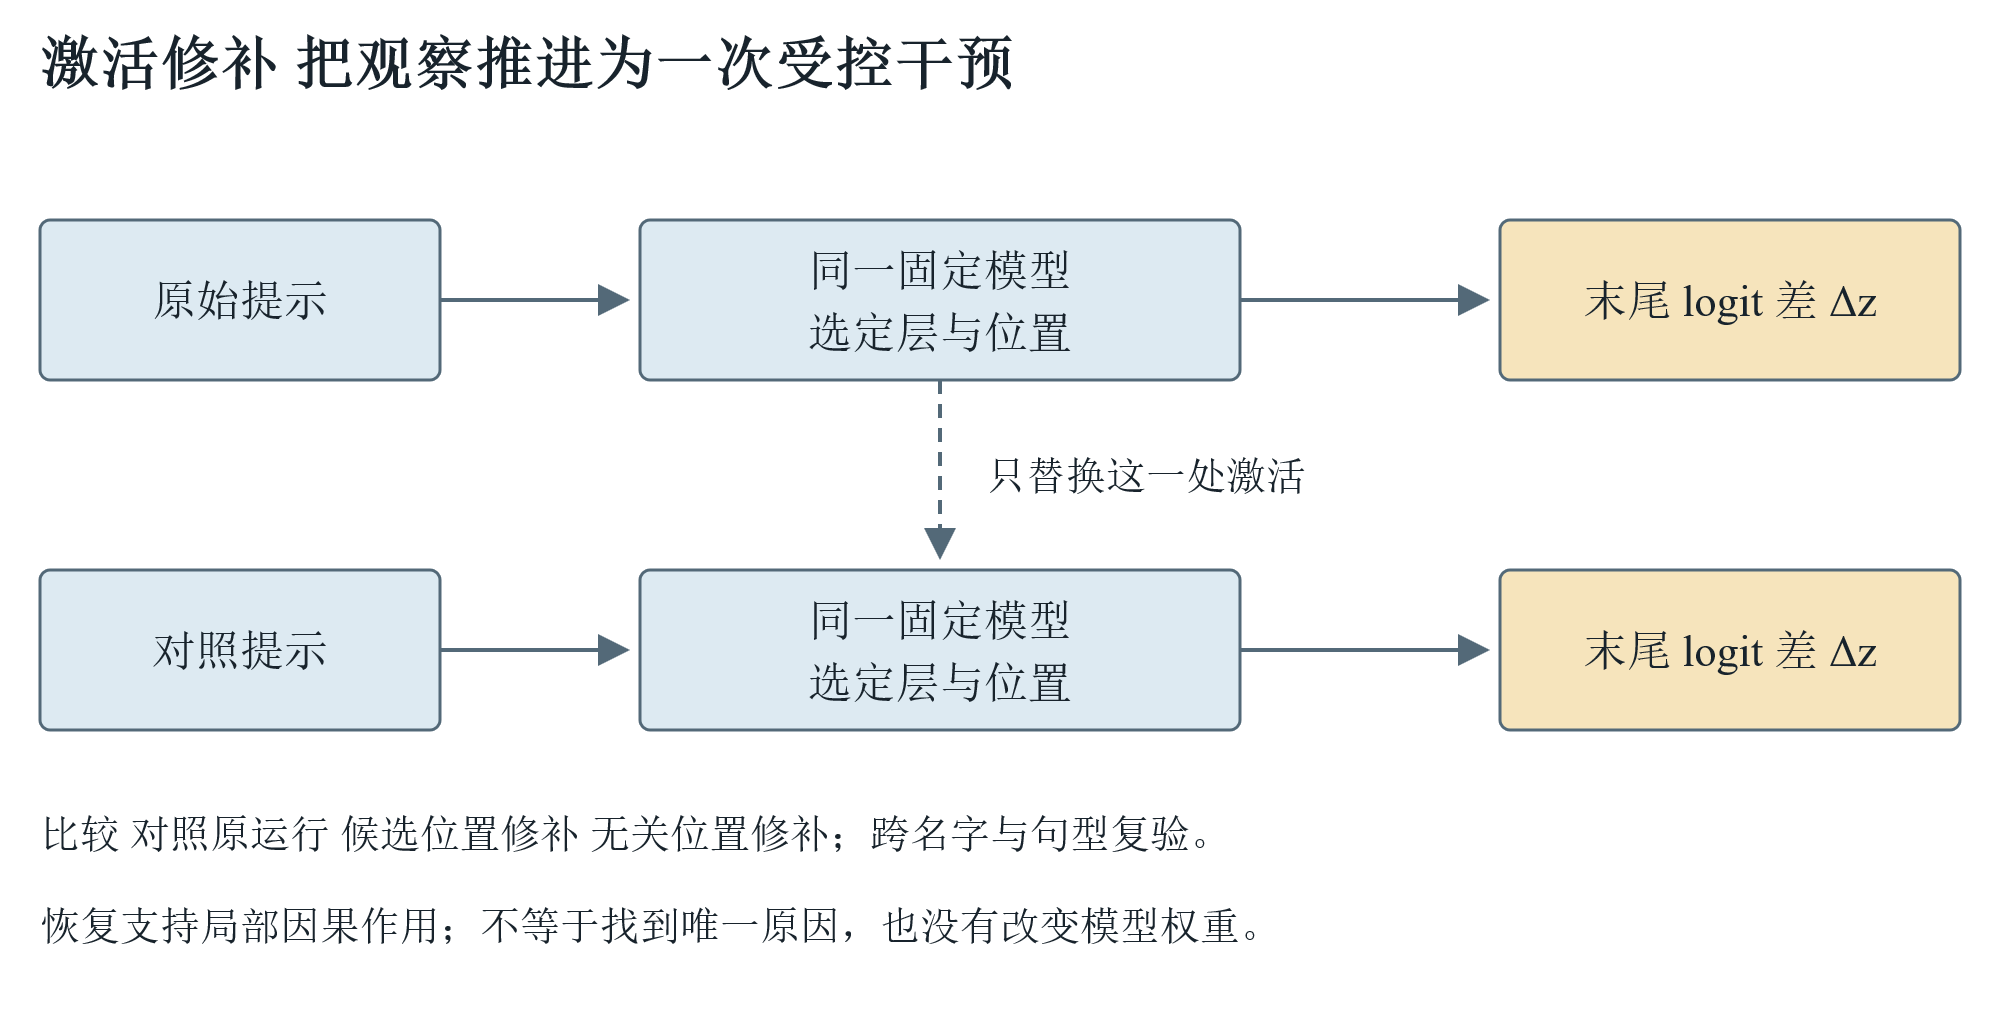
\includegraphics[width=\linewidth]{assets/media/image22.png}
    \caption{激活修补的受控实验。虚线表示将原始运行的指定激活替换到对照运行中；无关位置的修补提供负对照。}
    \label{fig:激活修补实验}
\end{figure}


\textbf{用三次运行计算恢复程度}~一次候选位置实验包含原始运行、对照运行和修补运行。假设三次运行的 Bob 与 Alice 分数差分别是 4、$-2$ 和 1。对照输入原本偏向 Alice，修补后转向 Bob。可以定义归一化恢复分数
\[
\rho=\frac{\Delta z_{\mathrm{patch}}-\Delta z_{\mathrm{ctrl}}}
{\Delta z_{\mathrm{orig}}-\Delta z_{\mathrm{ctrl}}}.
\]
$\Delta z_{\mathrm{orig}}$、$\Delta z_{\mathrm{ctrl}}$、$\Delta z_{\mathrm{patch}}$ 分别是原始、对照和修补运行的 logit 差，$\rho$ 表示修补填补了多少原始与对照之间的分数差距。上例中 $\rho=(1-(-2))/(4-(-2))=0.5$，即恢复了差距的 50\%。$\rho=0$ 表示与对照相同，$\rho=1$ 表示达到原始分数差；负值表示朝相反方向移动，大于 1 表示超过原始分数差。这个比值要求两条基线之间存在清晰差异，实验同时报告三次运行的原始分数，便于理解恢复幅度。

逐层、逐位置重复修补，可以画出恢复分数热图。比如某个位置在中间几层反复得到较高分数，就优先检查该位置相关的注意力头或前馈网络。随后在新句型上复验，并与无关位置修补、相同输入自修补比较，将候选范围缩小到具体计算组件。

图 \ref{fig:激活修补实验} 中，两次运行共享全部权重。竖向虚线只替换一个明确指定的中间状态；其后计算继续使用对照输入的其余状态。记录干预前后的 logit 差，可以量化修补对候选倾向的影响，并比较多个输入上的效果。

如果一个位置的修补稳定恢复了倾向，我们获得了``在这组输入和干预方式下，这处状态携带了影响输出的信息''的证据。接下来更换名字、句型与对照方式复验，并修补无关位置作负对照。源激活与目标位置按角色和位置对齐，使替换后的状态与当前计算保持可比较的语义条件。

我们再用消融（ablation）检查另一侧：移除、替换为均值或重采样某个组件的输出，行为是否受损？移除、均值替换和重采样分别改变组件输出的不同统计性质，实验记录具体操作并比较效果。对于多条路径共同完成的行为，可以组合消融多个组件，检验路径之间的补偿关系。把组件、连接和信息传递顺序组织起来，就形成可重复检验的计算回路（circuit）假设。

\textbf{本节相关资料}
\begin{enumerate}
    \item Wang 等，2022，\href{https://arxiv.org/abs/2211.00593}{Interpretability in the Wild A Circuit for Indirect Object Identification in GPT-2 small} 。阅读重点：怎样把一个可控行为分解成候选组件与计算路径。
    \item Zhang 与 Nanda，2023，\href{https://arxiv.org/abs/2309.16042}{Towards Best Practices of Activation Patching in Language Models Metrics and Methods} 。阅读重点：对照构造、度量和修补方式为什么会改变结论。
\end{enumerate}

\section{叠加表示与稀疏自编码器~一个神经元未必对应一个概念}\label{叠加表示与稀疏自编码器 一个神经元未必对应一个概念}

做完修补，我们查看一个候选神经元的高激活文本，发现它既回应课程说明，也回应某些代码片段。这些输入共享哪些特征，需要结合更多激活样本分析。模型中的特征可以沿多个神经元共同构成的方向表示，因此单个坐标上的激活会混合多种信息。

叠加表示（superposition）研究一种可能性：许多特征利用不完全正交的方向共享有限维度。当每次只出现少量相关特征时，这种共享可能仍有用。这种表示方式使同一个神经元参与多个特征的编码。分析时可以从多个坐标构成的方向入手，寻找在不同输入中稳定出现的激活模式。

\textbf{用二维例子理解特征共享}~假设模型只有两个表示维度，却要编码三种特征。为三种特征选择方向 $u_1=(1,0)$、$u_2=(0,1)$、$u_3=(1,1)/\sqrt2$，再把一次输入的表示写成
\[
h=a_1u_1+a_2u_2+a_3u_3.
\]
这里，$h$ 是二维表示，$u_1,u_2,u_3$ 是三个单位特征方向，$a_1,a_2,a_3$ 是当前输入中各特征的强度。如果每次只有一种特征出现，三个方向可以分别表示三种模式；第三种特征出现时，两个坐标都会激活。如果多种特征同时出现，方向之间会相互干扰。稀疏性意味着每个输入通常只使用少量特征，使共享维度成为一种节省表示容量的方式。

稀疏自编码器（Sparse Autoencoder，SAE）尝试把某层激活重新表示为一个更大的、但每次只激活少数项的特征向量。编码器把原激活 h 映射为特征 f(h)，解码器再重建出 h 的估计值。一个便于理解的训练目标，同时惩罚重建误差与特征激活的绝对值之和：
\[L_{SAE} = E_{h}\left\lbrack \lVert h-\widehat h\rVert_2^2 + \lambda \parallel f(h) \parallel_{1} \right\rbrack\]

这里 h 是收集到的模型激活，h 上的帽号是重建值，第一项是平方重建误差；第二项的 1 范数表示各特征激活绝对值之和，λ 控制稀疏程度。这个 L1 型目标通过激活惩罚鼓励稀疏表示；训练时同时约束解码向量尺度，使惩罚反映特征使用程度。其他 SAE 设计也可以通过限制激活数量等方式实现稀疏性。训练 SAE 时，原模型保持冻结。

\textbf{编码器和解码器具体做什么}~一个基础的 ReLU 型 SAE 可以写成
\[
f(h)=\operatorname{ReLU}(W_{\mathrm{enc}}h+b_{\mathrm{enc}}),
\qquad \widehat h=W_{\mathrm{dec}}f(h)+b_{\mathrm{dec}}.
\]
这里，$h\in\mathbb R^d$ 是原模型的 $d$ 维激活，$f(h)\in\mathbb R^m$ 是 SAE 的特征激活，通常选择 $m>d$。$W_{\mathrm{enc}}\in\mathbb R^{m\times d}$ 和 $b_{\mathrm{enc}}\in\mathbb R^m$ 是编码器权重与偏置；$\operatorname{ReLU}$ 把每个负值置零，正值保留。$W_{\mathrm{dec}}\in\mathbb R^{d\times m}$ 和 $b_{\mathrm{dec}}\in\mathbb R^d$ 是解码器权重与偏置，把特征激活重建为 $\widehat h$。解码矩阵的第 $j$ 列给出第 $j$ 个特征写回原表示空间的方向。

例如，原隐藏向量有 768 维，SAE 可以扩展到 6144 个候选特征，并通过稀疏约束让每个输入只使用其中少量特征。一个假想样本的非零特征激活为 1.2、0.7、0.4，其 L1 惩罚中的激活绝对值之和就是 2.3。若平方重建误差为 0.2，$\lambda=0.1$，该样本的总损失为 $0.2+0.1\times2.3=0.43$。重建项推动 SAE 保留原激活的信息，稀疏项推动它用更少的特征完成重建；提高 $\lambda$ 会加强对特征激活的惩罚。

\textbf{SAE 也需要训练，训练目标来自激活本身}~研究者先选择模型层与读取位置，收集大量文本在这些位置产生的激活向量。冻结原模型后，随机初始化 SAE 的编码器与解码器，按批次计算重建值和损失，用梯度下降更新 SAE 的权重与偏置，并维持解码向量的尺度约束。损失中的 $E_h$ 表示对收集的激活样本取平均。这里每个样本的重建目标就是原向量 $h$，采用自监督重建训练；9.2 的探针则使用事先标注的类别作为监督目标。

训练完成后，按每个特征的激活强度排列文本位置，观察得分最高的上下文。例如，某个特征在 Python 的 def、return 及函数体附近频繁激活，就可以提出与函数定义相关的描述，再用新代码与普通文本检查这个描述。特征名称在分析阶段根据样本提出，SAE 训练阶段学习的是稀疏重建。

还可以沿单个特征的解码方向修改原模型激活：
\[
h'=h+\alpha w_j.
\]
这里，$w_j$ 是 $W_{\mathrm{dec}}$ 的第 $j$ 列，$\alpha$ 是研究者设定的干预强度，$h'$ 是修改后继续送入后续网络层的激活。改变 $\alpha$ 并记录下一 token 概率或任务表现，可以研究这个特征方向对生成行为的影响。激活修补从另一条运行中取得完整状态，SAE 特征干预则围绕学到的单个方向调整状态，两种操作提供不同粒度的实验手段。

如果若干特征更容易用一致的文本模式描述，我们获得了更便于分析的坐标系。研究者根据高激活样本为特征提出描述，再用新数据检查描述的覆盖范围，比较反例与重建质量，并通过特征干预检验行为预测。特征数量与稀疏程度影响表示的粒度：较大的特征集合可以细分模式，训练数据的覆盖则影响稀有模式的提取。

例如，某个特征在如实报告已知事实的回答中频繁激活，研究者可以将其描述为与诚实回答相关的候选特征。随后在事实问答、信息不足和存在误导提示等场景中调节该特征，记录准确率、不确定性表达和回答风格的变化。特征描述、干预效果与跨任务评估共同构成对这个候选特征的机制分析。

\textbf{本节相关资料与研究材料}
\begin{enumerate}
    \item Elhage 等，2022，\href{https://arxiv.org/abs/2209.10652}{Toy Models of Superposition} 。阅读重点：在可控玩具模型里，稀疏性与特征共享如何相互影响。
    \item Gao 等，2024，\href{https://arxiv.org/abs/2406.04093}{Scaling and evaluating sparse autoencoders} 。阅读重点：稀疏程度、重建质量与评估如何权衡。
\end{enumerate}

\section{最小解释实验 从一个问题走到可复核的结论}\label{最小解释实验 从一个问题走到可复核的结论}

我们把可解释性入门收束成一次小实验，目标是解释一个具体行为：在某类人物关系句子上，哪些中间状态影响下一名字的选择？我们选用可访问中间激活的小型 Transformer，先确保基线行为足够稳定，再开始分析。

第一步建立一小批原始与对照提示，按句型分出开发组和未见测试组。记录 tokenizer、模型检查点、候选 token、位置对齐方式与基线 Δz。根据基线表现选择模型能够稳定完成的句型，使原始与对照输入形成清晰的输出差异。

第二步只选择一种激活类型，例如每层指定位置的残差流（residual stream，即各组件输出通过残差连接累加的表示），逐处缓存与修补。每次只改一个对象，保存输入、源激活、目标位置和输出分数。各位置的恢复分数用于筛选影响较大的候选层与位置，为下一步复验确定范围。

第三步固定筛出的少量候选，在未见名字与句型上复验，加入无关位置和相同输入自修补等控制。检查效果是否依赖一个特殊对照，是否牺牲其他行为。需要时再补线性探针或细分到注意力头。每轮实验固定任务、模型和指标，逐项改变干预位置或方式，便于追踪效果来源。

我们可以把实验计划写成一张紧凑记录表：

\begin{longtable}[]{@{}
  >{\raggedright\arraybackslash}p{(\linewidth - 4\tabcolsep) * \real{0.2985}}
  >{\raggedright\arraybackslash}p{(\linewidth - 4\tabcolsep) * \real{0.2985}}
  >{\raggedright\arraybackslash}p{(\linewidth - 4\tabcolsep) * \real{0.4030}}@{}}
\toprule\noalign{}
\begin{minipage}[b]{\linewidth}\raggedright
\textbf{环节}
\end{minipage} & \begin{minipage}[b]{\linewidth}\raggedright
\textbf{固定或记录的内容}
\end{minipage} & \begin{minipage}[b]{\linewidth}\raggedright
\textbf{通过条件}
\end{minipage} \\
\midrule\noalign{}
\endhead
\bottomrule\noalign{}
\endlastfoot
行为基线 & 原始与对照提示 候选及 token 切分 & 目标倾向有可测量差异 \\
候选筛选 & 激活类型 层与位置 修补来源 & 效果超过无关位置控制 \\
独立复验 & 新实体 新句型 另一种对照 & 方向与预设假设一致 \\
结论范围 & 模型版本 任务与干预定义 & 结论明确对应所测输入与干预结果 \\
\end{longtable}

最后写报告时，我们把``事实观察''\,``机制假设''\,``未排除的解释''分开。一个清楚的结论可以是：``在该模型和这类句子上，把第某层某位置的原始残差激活移入对照运行，会使候选分数差向原始方向移动。''结论写明模型、输入、干预位置与输出变化，其他研究者就能按相同步骤复查，并用新的输入检验机制假设。

我们现在可以把这一章接回训练诊断。内部分析能帮助提出新假设，比如输出头是否改变、某条纠错路径是否受损；根据这些假设实施修复后，再用独立题集衡量任务收益，用旧能力回归检查行为变化，并记录计算成本。内部机制分析负责定位和解释计算变化，行为评估负责衡量变化带来的实际效果，两类结果共同指导下一轮模型改进。

\textbf{本节相关资料}
\begin{enumerate}
    \item Zhang 与 Nanda，2023，\href{https://arxiv.org/abs/2309.16042}{Towards Best Practices of Activation Patching in Language Models Metrics and Methods} 。阅读重点：把输入构造与度量选择纳入实验报告。
    \item Wang 等，2022，\href{https://arxiv.org/abs/2211.00593}{Interpretability in the Wild A Circuit for Indirect Object Identification in GPT-2 small} 。阅读重点：从候选筛选走向可重复验证的回路假设。
\end{enumerate}
